\documentclass[12pt,a4paper]{report}
\setlength\textwidth{145mm}
\setlength\textheight{247mm}
\setlength\oddsidemargin{15mm}
\setlength\evensidemargin{15mm}
\setlength\topmargin{0mm}
\setlength\headsep{0mm}
\setlength\headheight{0mm}
\setlength{\parindent}{4em}

\let\openright=\clearpage


\usepackage[czech]{babel}

\usepackage[utf8]{inputenc}

\usepackage{indentfirst}
\usepackage{graphicx}
\usepackage{color}
\usepackage{pdfpages}

\usepackage{amsthm}
\usepackage{setspace}

\usepackage[unicode]{hyperref}  
\hypersetup{pdftitle=Název práce}
\hypersetup{pdfauthor=Jméno Příjmení}


\makeatletter
\def\@makechapterhead#1{
  {\parindent \z@ \raggedright \normalfont
   \Huge\bfseries \thechapter. #1
   \par\nobreak
   \vskip 20\p@
}}
\def\@makeschapterhead#1{
  {\parindent \z@ \raggedright \normalfont
   \Huge\bfseries #1
   \par\nobreak
   \vskip 20\p@
}}
\makeatother


\def\chapwithtoc#1{
\chapter*{#1}
\addcontentsline{toc}{chapter}{#1}
}

\begin{document}


\lefthyphenmin=2
\righthyphenmin=2


\pagestyle{empty}
\begin{center}

\large

{\bf ČESKÁ ZEMĚDĚLSKÁ UNIVERZITA V PRAZE}

\medskip

FAKULTA ŽIVOTNÍHO PROSTŘEDÍ

\vfill

\vfill

{\bf \Large BAKALÁŘSKÁ PRÁCE}

\vfill

\vspace{10cm}

\vfill


\hbox{\hbox to 0.5\hsize{%
2018
\hss}\hbox to 0.5\hsize{%
\hspace{100pt} Irina Georgievová
\hss}}

\end{center}
\pagestyle{empty}
\newpage
\begin{center}

\large

{ \bf ČESKÁ ZEMĚDĚLSKÁ UNIVERZITA V PRAZE}

\medskip

FAKULTA ŽIVOTNÍHO PROSTŘEDÍ

\medskip

{\sc \Large katedra vodního hospodářství a~environmentálního modelování}

\vfill

\vfill

{\LARGE Vizualizace enviromentálních dat}

\vspace{2mm}

{\bf \Large BAKALÁŘSKÁ PRÁCE}

\vspace{15mm}

\vfill

\vfill

\begin{tabular}{rl}

\noalign{\vspace{2mm}}
Vedoucí práce: & \bf doc. Ing. Martin Hanel, Ph.D. \\
\noalign{\vspace{2mm}}
Bakalant: & \bf Irina Georgievová \\
\end{tabular}

\vfill

2018

\end{center}
\newpage
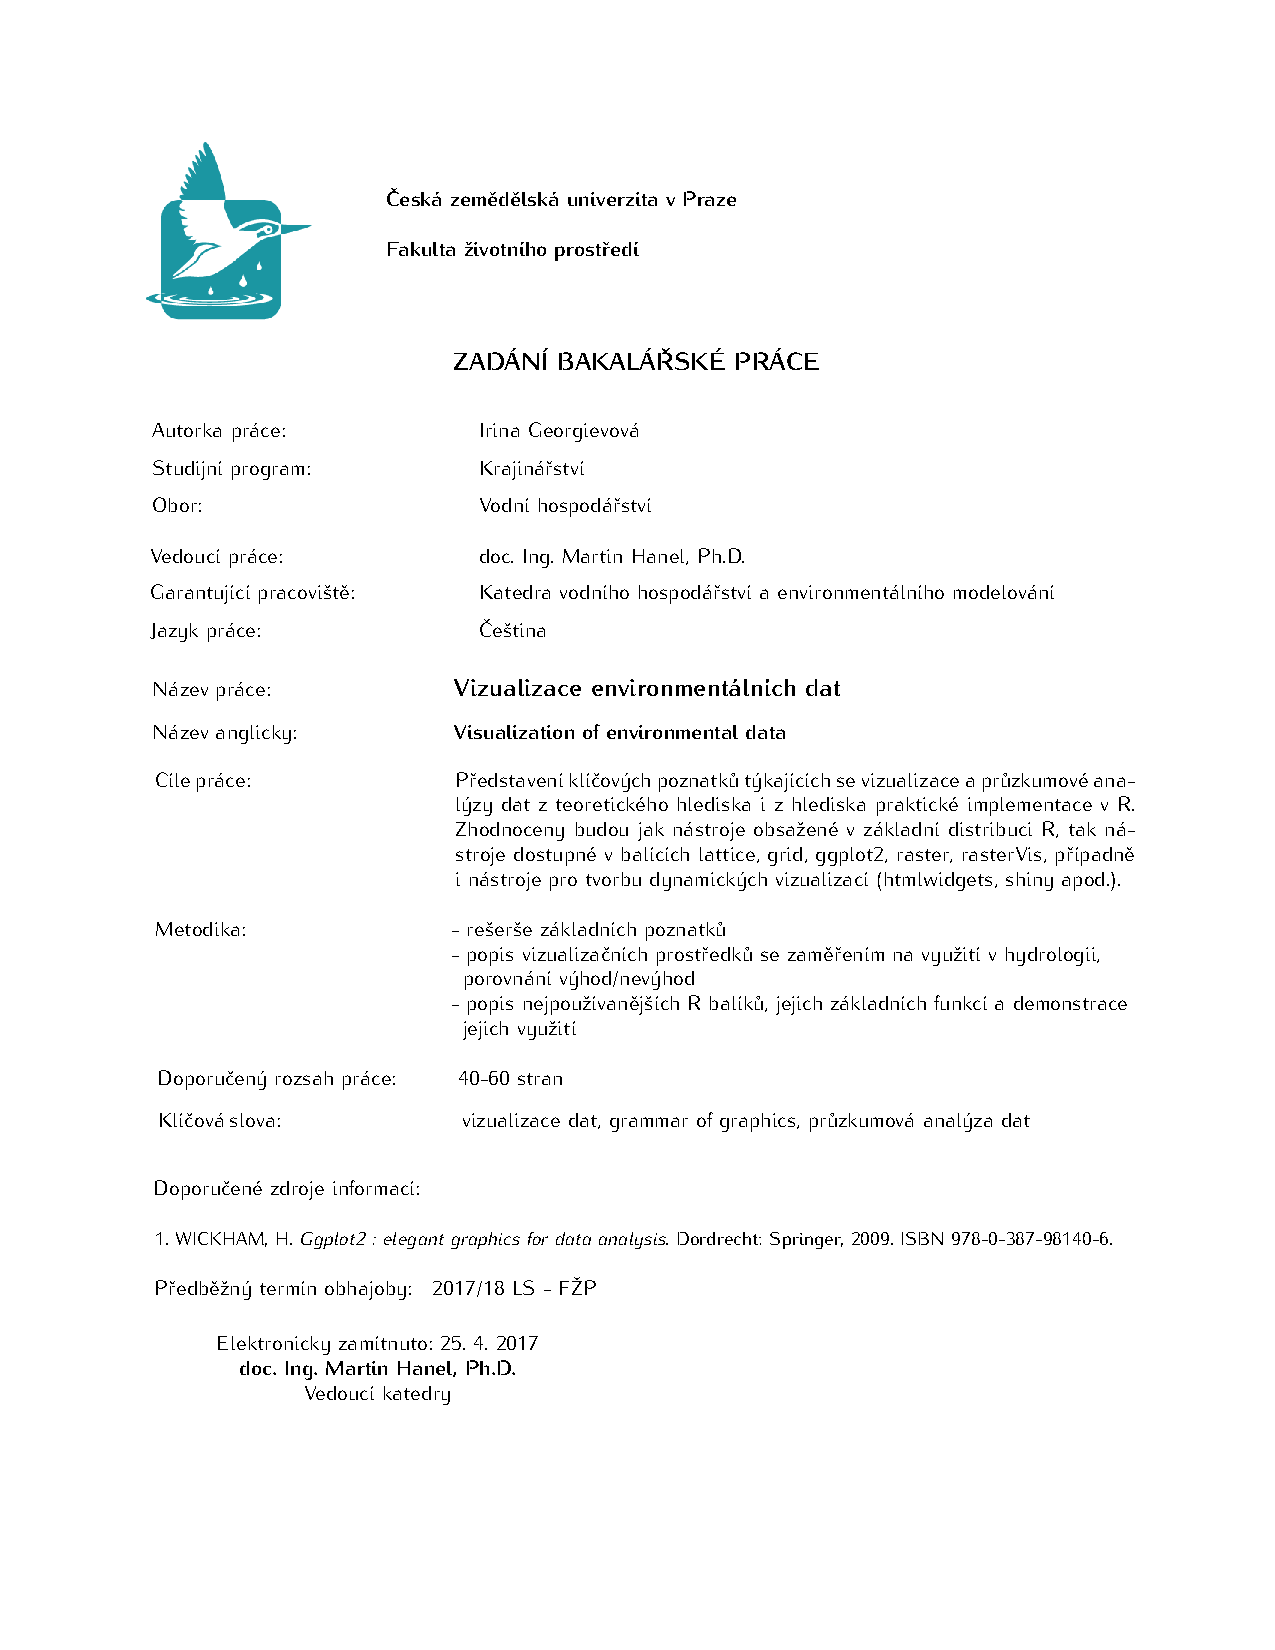
\includepdf[pages=1,pagecommand={}]{zadani.pdf}
\newpage


\vglue 0pt plus 1fill

\noindent
{\bfseries Prohlášení:} \\
Prohlašuji, že jsem bakalářskou práci \emph{Vizualizace enviromentálních dat} zpracovala samostatně. Veškerou literaturu a další podkladové materiály uvádím v~ seznamu na straně %~\pageref{literatura}.

\vspace{10mm}

\hbox{\hbox to 0.5\hsize{%
V Praze dne ..................
\hss}\hbox to 0.5\hsize{%
\hspace{100pt}...........................
\hss}}

\vspace{1mm}
\hbox{\hbox to 0.5\hsize{%

\hss}\hbox to 0.5\hsize{%
\hspace{100pt}Irina Georgievová
\hss}}

\vspace{20mm}

\newpage

\vglue 0pt plus 1fill
\noindent
{\bfseries Poděkování:} \\

\newpage

\newpage


\vbox to 0.5\vsize{
\setlength\parindent{0mm}
\setlength\parskip{5mm}

{\LARGE\bfseries Abstrakt} 

Vložte abstrakt o rozsahu cca 100–200 slov. K problému vícenásobné marginalizace (VM) dochází, pokud články dodavatelského řetězce nastavují cenu svého výstupu způsobem, který by optimalizoval zisk v podmínkách prodávajícího na trhu s koncovým zbožím. V takové situaci dochází k cenové spirále a výsledná cena koncové produkce svou přílišnou výší poškozuje jak spotřebitelský užitek, tak i zisk řetězce jako celku. Kvantifikace dopadu VM byla již předmětem našeho dřívějšího výzkumu. Tento příspěvek se zabývá otázkou, za jakých podmínek k cenové spirále dochází a jakým způsobem probíhá konvergence k výsledným (rovnovážným) cenám. Pro tyto účely byl navržen a implementován model řetězce v podobě multiagentního systému, se kterým je možné analyzovat celý proces pomocí počítačové simulace.


{\bfseries Klíčová slova: } vizualizace dat, grammar of graphics, průzkumová analýza dat
\vss}\nobreak\vbox to 0.49\vsize{
\setlength\parindent{0mm}
\setlength\parskip{5mm}
{\LARGE\bfseries Abstract} 

Double (or multiple) marginalization is often identified as the main source of a decentralized supply chain’s (SC’s) inefficiency. In its core lies the fact that if the agents constituting the SC choose their output prices according to the golden rule of profit maximization (which normally applies to a single firm that produces independently and sells directly to the end consumer), the prices in the SC tend to spiral up to an inefficient level (equilibrium prices) where both the consumer surplus and the SC’s total profit are diminished. The level of equilibrium prices and their impact on the SC’s profit and efficiency had been studied in our earlier works. Our focus in this paper was the properties of the process of convergence of the prices inside the SC to equilibrium levels. The analysis was carried out using computer experiments with an agent-based simulation model of a SC with limited information. Only serial chain structure was considered.

{\bfseries Keywords:  } Data visualization, grammar of graphics, exploratory data analysis
\vss}

%\newpage
%
%
%\openright
%\pagestyle{plain}
%\setcounter{page}{1}
%\tableofcontents
%
%\chapter*{Úvod}
%\addcontentsline{toc}{chapter}{Úvod}
%\setstretch{1.25}
%Double (or multiple) marginalization is often identified as the main source of a decentralized supply chain’s (SC’s) inefficiency. In its core lies the fact that if the agents constituting the SC choose their output prices according to the golden rule of profit maximization (which normally applies to a single firm that produces independently and sells directly to the end consumer), the prices in the SC tend to spiral up to an inefficient level (equilibrium prices) where both the consumer surplus and the SC’s total profit are diminished. The level of equilibrium prices and their impact on the SC’s profit and efficiency had been studied in our earlier works. Our focus in this paper was the properties of the process of convergence of the prices inside the SC to equilibrium levels. The analysis was carried out using computer experiments with an agent-based simulation model of a SC with limited information. Only serial chain structure was considered.
%\chapter{Název první kapitoly}
%
%\section{Název první podkapitoly v první kapitole}
%
%\section{Název druhé podkapitoly v první kapitole}
%
%
%\chapter{Název druhé kapitoly}
%
%\section{Název první podkapitoly v druhé kapitole}
%
%\section{Název druhé podkapitoly v druhé kapitole}
%
%
%\chapter*{Závěr}
%\addcontentsline{toc}{chapter}{Závěr}
%
%
%\def\bibname{Literatura}
%\setstretch{1}
%\begin{thebibliography}{99}\label{literatura}
%
%\addcontentsline{toc}{chapter}{\bibname}
%
%\bibitem{Charlier2006}
% {\sc Charlier} Isabelle, 
% {\sc Paindaveine} Davy,
% {\sc Saracco} Jer\^{o}me.
% {Conditional quantile estimation based on optimal quantization:} 
% {From theory to practice.}
% {\em Computational Statistics \& Data Analysis} 
% {\bf 91}, 
% {2015,} 
% {20--39.}
%
%\bibitem{lamport1994}
% {\sc Lamport} Leslie.
% \emph{A Document Preparation System.}
% {2.~vydání}.
% {Massachu\-setts:~Addison Wesley,} 
% {1994.}
% {ISBN 0-201-52983-1.}
%
%\end{thebibliography}
%
%
%
%\chapwithtoc{Seznam tabulek}
%
%\chapwithtoc{Seznam zkratek}
%
%\chapwithtoc{Přílohy}
%
%\openright
\end{document}
